% 三矢量的混合积

\pentry{矢量的叉乘\upref{Cross}}
\subsection{定义}

任意的三个矢量,如果其中两个叉乘再与第三个矢量点乘,那么这种运算叫做这三个矢量的\textbf{混合积}

$\vec A \cross \vec B \vdot \vec C$ 是矢量 $\vec A$, $\vec B$, $\vec C$ 的混合积,且满足
\begin{equation}\label{TriVM_eq1}
\vec A \cross \vec B \vdot \vec C = \vec B \cross \vec C \vdot \vec A = \vec C \cross \vec A \vdot \vec B 
\end{equation} 
这个公式可由下图记忆.
\begin{figure}[ht]
\centering
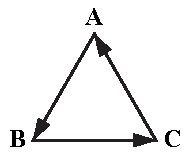
\includegraphics[width=0.25\textwidth]{./figures/TriVM.pdf}
\caption{\autoref{TriVM_eq1} 记忆法}
\end{figure}
混合积的方向由叉乘的方向决定,与点乘无关.如果混合积的顺序取与右图相反的方向,根据叉乘的定义,需要在前面加上负号(叉乘不满足乘法交换律!).下面三式与上面三式互为相反数.
\begin{equation}
\vec C \cross \vec B \vdot \vec A = \vec B \cross \vec A \vdot \vec C = \vec A \cross \vec C \vdot \vec B
\end{equation} 
另外要注意混合积的方向是由叉乘的次序所决定的,与点乘的次序无关.所以上式也可记为
 \begin{equation}
\vec A \vdot (\vec C \cross \vec B) = \vec C \vdot (\vec B \cross \vec A) = \vec B \vdot (\vec A \cross \vec C)
\end{equation} 
注意括号是必须的, $\vec A \vdot \vec C \cross \vec B$ 是错误的式子,因为 $\vec A \vdot \vec C$ 是常数,不能与 $\vec B$ 叉乘.


\subsection{几何法证明}

设三个矢量都以原点作为起点,以三个矢量为棱作平行六面体(如图,%未完成:引用图片
).从矢量的叉乘\upref{Cross}可知 $\abs{\vec A \cross \vec B}$ 就是 $\vec A,\vec B$,  所在平行四边形的面积.令 $\vec A \cross \vec B = \abs{\vec A \cross \vec B} \uvec n$, 则 $\uvec n$ 为平面的法向量.平行六面体的高为 $\abs{\uvec n \vdot \vec C}$, 所以平行六面体的体积为底面积乘以高
\begin{equation}
V = \abs{\vec A \cross \vec B} \abs{\uvec n \vdot \vec C} = \abs{\vec A \cross \vec B \vdot \vec C}
\end{equation}
同理可得对于同一平行六面体
\begin{equation}
V = \abs{\vec B \cross \vec C \vdot \vec A} = \abs{\vec C \cross \vec A \vdot \vec B} 
\end{equation}  
这里只证明了绝对值,证明正负关系并不难,留给读者思考.

\subsection{代数法证明}
不难证明三矢矢积若展开成分量的形式,等于三个矢量组成的行列式.而利用行列式中任意两行置换符号改变,即可证明\autoref{TriVM_eq1}


